% Automatski generisano skriptom assignment7_analysis.py.
\section{Eksperiment i analiza rezultata}

Waypoint misija je izvršena u tri konfiguracije propisane zadatkom: (a) regulator zatvoren preko odometrije, (b) regulator zatvoren preko EKF estimacije sa uključenom popravkom i (c) regulator zatvoren preko EKF estimacije bez popravke. Za analizu praga validacije dodatno se ponavlja konfiguracija (b) za više vrednosti praga $g$.

\subsection{Poređenje trajektorija}
\begin{figure}[h]
\centering
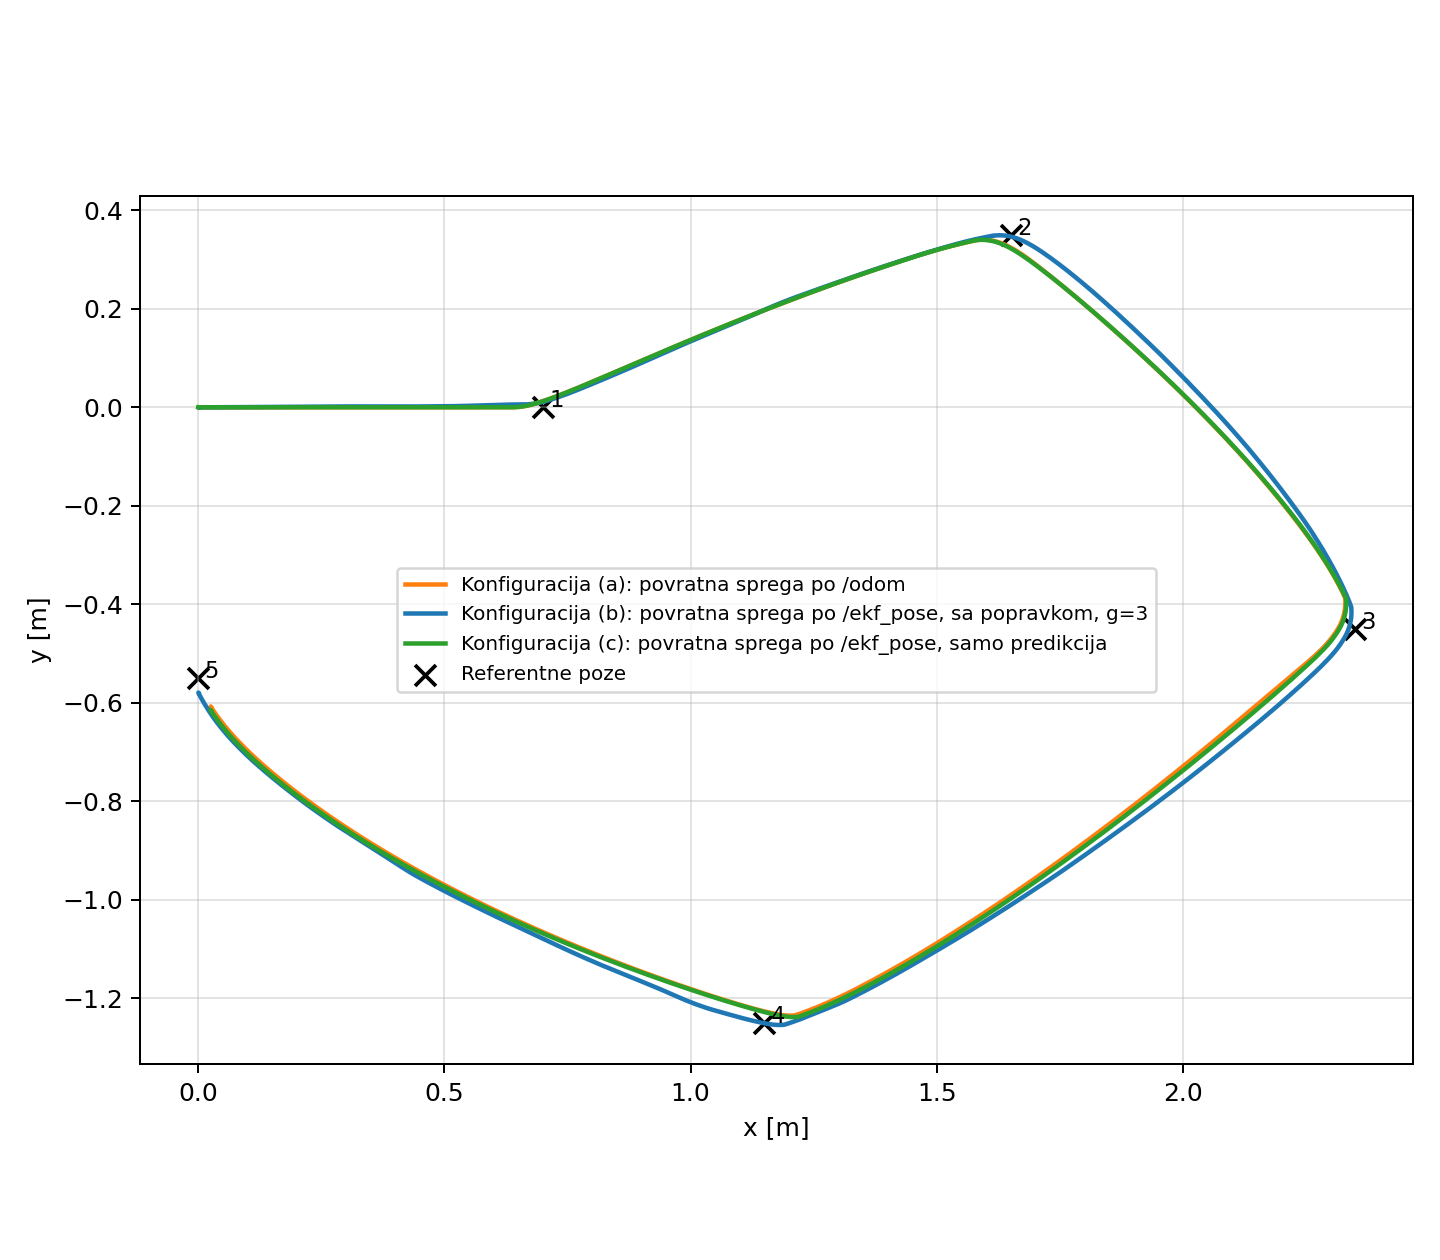
\includegraphics[width=0.92\linewidth]{results/figures/assignment7_trajectories.png}
\caption{Ground truth putanje robota za tri konfiguracije i zadate referentne poze.}
\end{figure}

\begin{figure}[h]
\centering
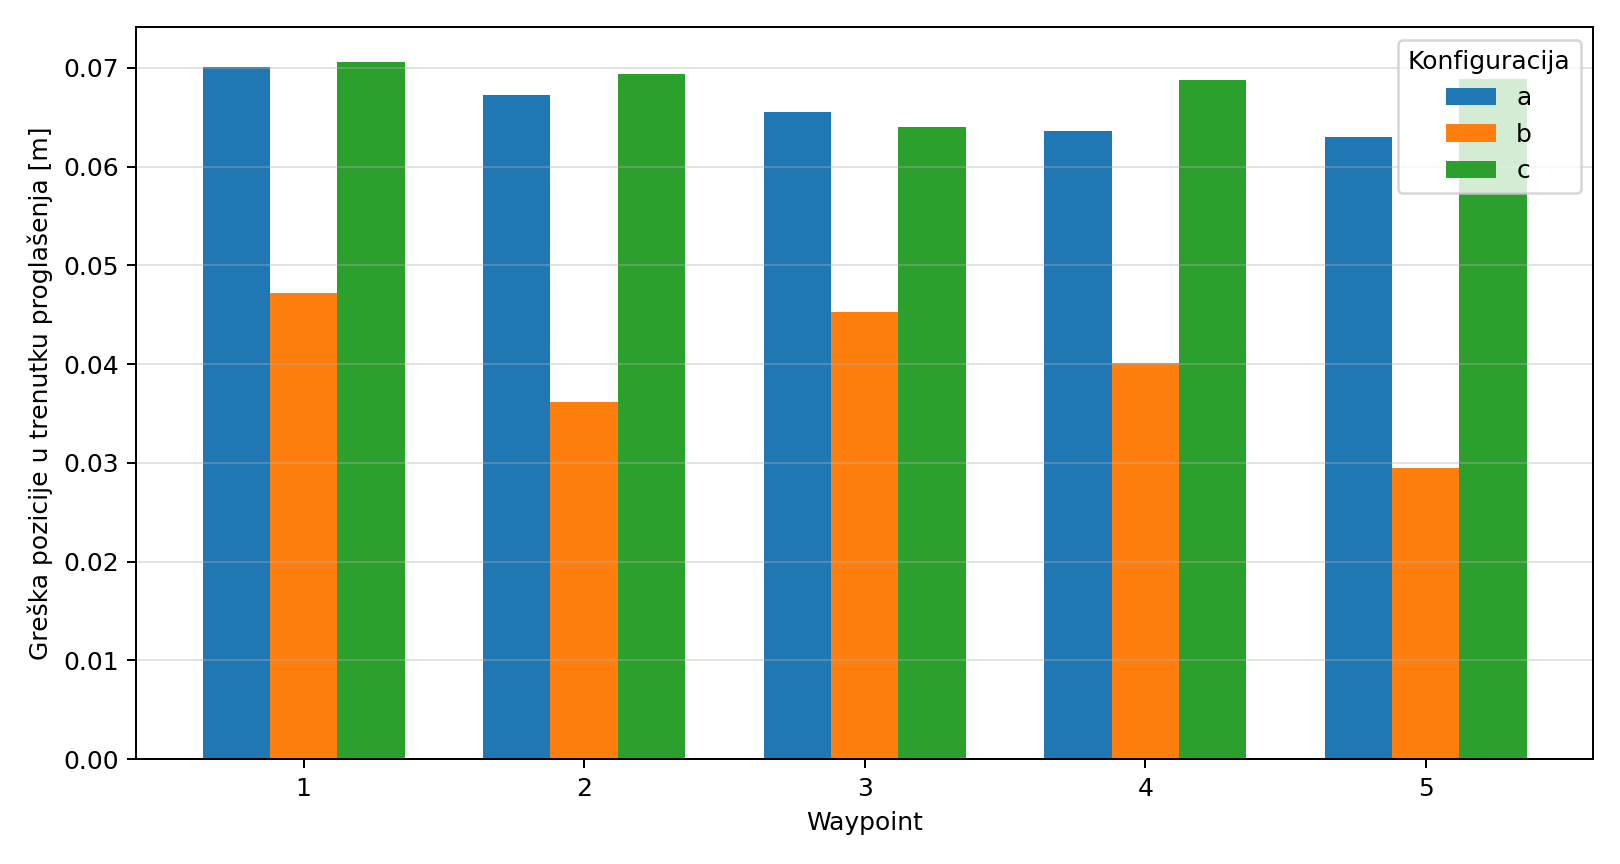
\includegraphics[width=0.86\linewidth]{results/figures/assignment7_waypoint_errors.png}
\caption{Rastojanje ground truth poze od reference u trenutku kada regulator proglasi waypoint dostignutim.}
\end{figure}

Srednja greška dostizanja referentne poze iznosi \SI{0.066}{m} za konfiguraciju (a), \SI{0.040}{m} za konfiguraciju (b) i \SI{0.068}{m} za konfiguraciju (c). U ovom eksperimentu EKF sa popravkom smanjuje srednju grešku dostizanja za 39.8\% u odnosu na upravljanje po odometriji i za 42.0\% u odnosu na EKF bez popravke. To potvrđuje da se u zatvorenoj petlji ne dobija samo lepša estimacija, već i tačnije zaustavljanje robota u referentnim pozama.

\begin{table}[h]
\centering
\begin{tabular}{lrrrrr}
\hline
Konf. & $g$ & Srednja greška [m] & Maks. greška [m] & Trajanje [s] & Popravke \\
\hline
a & 3.0 & 0.066 & 0.070 & 36.7 & 183 \\
b & 3.0 & 0.040 & 0.047 & 37.4 & 187 \\
c & 3.0 & 0.068 & 0.071 & 35.9 & 0 \\
\hline
\end{tabular}
\caption{Sažetak uspešnosti waypoint misije za osnovne konfiguracije.}
\end{table}

Konfiguracije (a) i (c) pokazuju sličan oblik degradacije zato što se u oba slučaja upravljačka petlja oslanja na integraciju kretanja bez spoljašnje korekcije položaja. Kod (a) tu ulogu ima odometrija, a kod (c) EKF radi samo predikciju, pa akumulirana greška točkova ostaje neograničena.

\begin{table}[h]
\centering
\begin{tabular}{lrrr}
\hline
Konfiguracija & Waypoint & Greška pozicije [m] & Greška yaw [rad] \\
\hline
a & 1 & 0.070 & 0.000 \\
a & 2 & 0.067 & 0.086 \\
a & 3 & 0.066 & 0.073 \\
a & 4 & 0.064 & 0.088 \\
a & 5 & 0.063 & 0.090 \\
b & 1 & 0.047 & 0.006 \\
b & 2 & 0.036 & 0.132 \\
b & 3 & 0.045 & 0.091 \\
b & 4 & 0.040 & 0.085 \\
b & 5 & 0.030 & 0.082 \\
c & 1 & 0.071 & 0.000 \\
c & 2 & 0.069 & 0.087 \\
c & 3 & 0.064 & 0.080 \\
c & 4 & 0.069 & 0.077 \\
c & 5 & 0.069 & 0.086 \\
\hline
\end{tabular}
\caption{Tačnost dostizanja referentnih poza.}
\end{table}

\subsection{Greška estimacije}
\begin{figure}[h]
\centering
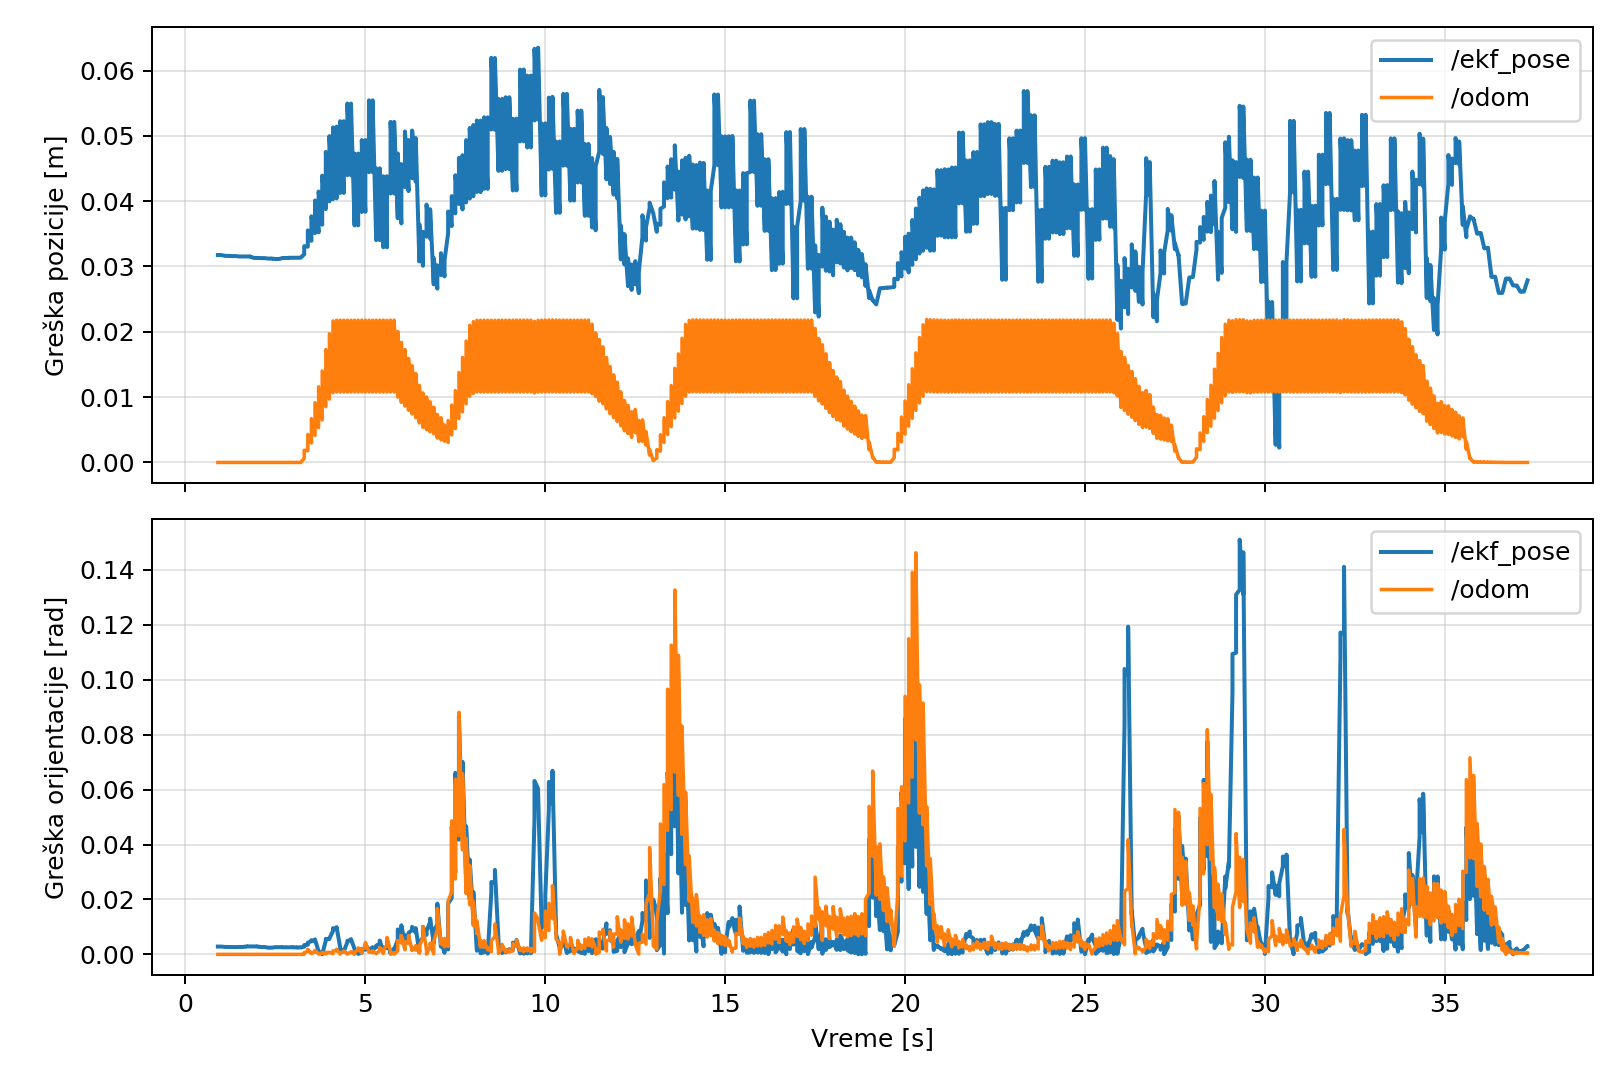
\includegraphics[width=0.92\linewidth]{results/figures/assignment7_estimation_error_b.png}
\caption{Greška pozicije i orijentacije za /ekf\_pose i /odom u odnosu na Gazebo ground truth, konfiguracija (b).}
\end{figure}

Za konfiguraciju (b) srednja greška pozicije EKF estimacije iznosi \SI{0.038}{m}, a maksimalna \SI{0.063}{m}. Odometrija u istoj vožnji ima srednju grešku \SI{0.011}{m} i maksimalnu \SI{0.022}{m}. Na ovoj kratkoj simulacionoj putanji odometrija ostaje veoma bliska ground truth pozi, što je očekivano jer simulator nema izražen proklizavajući drift. Ipak, waypoint metrika pokazuje da zatvaranje petlje po korigovanom EKF-u dovodi robota bliže referencama. Greška orijentacije EKF-a je srednje \SI{0.013}{rad}, dok je za odometriju \SI{0.012}{rad}.

\subsection{Evolucija kovarijanse}
\begin{figure}[h]
\centering
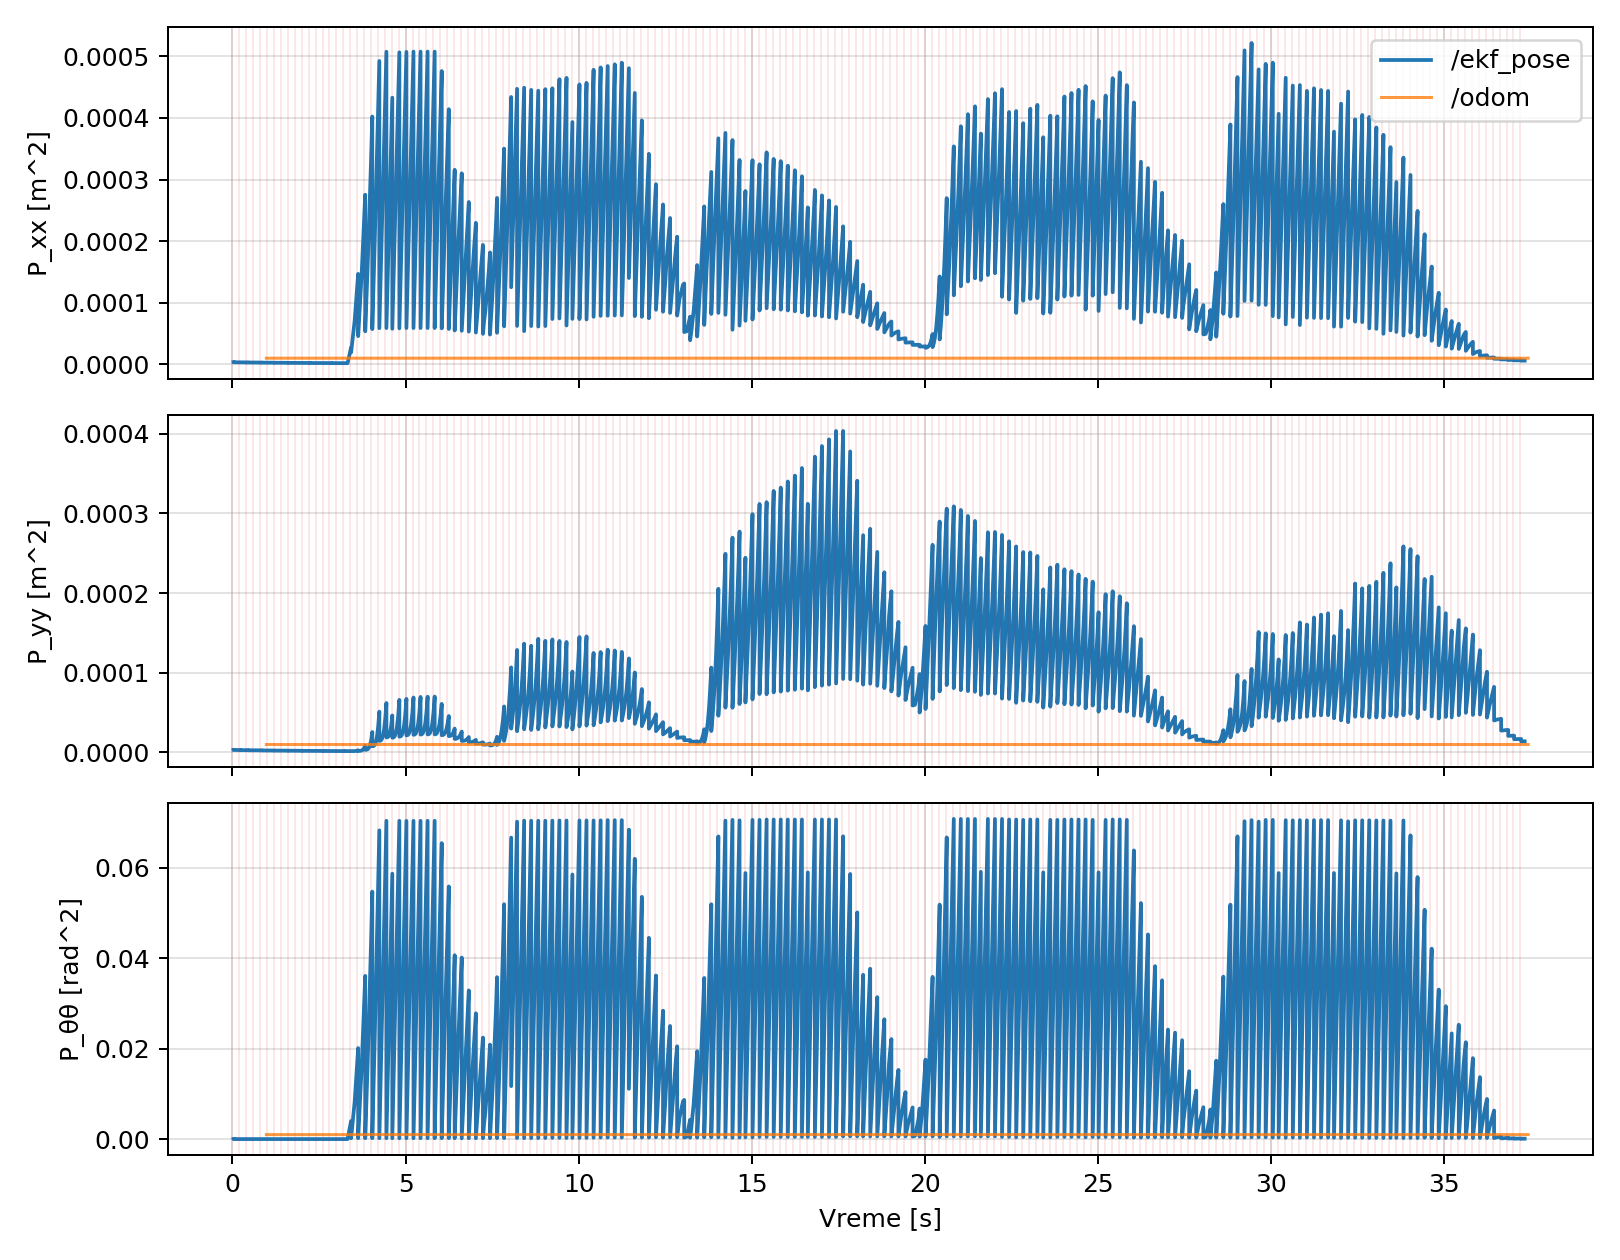
\includegraphics[width=0.92\linewidth]{results/figures/assignment7_covariance_b.png}
\caption{Dijagonalni elementi kovarijanse iz /ekf\_pose i /odom. Crvene vertikalne linije označavaju uspešne EKF popravke.}
\end{figure}

Srednje dijagonalne vrednosti EKF kovarijanse tokom konfiguracije (b) su približno $P_{xx}=0.0002$, $P_{yy}=0.0001$ i $P_{\theta\theta}=0.0242$. Na grafiku se vidi karakterističan obrazac: tokom predikcije kovarijansa raste, a pri uspešnim popravkama, označenim crvenim linijama, opada u komponentama koje opažene linije mogu da ograniče. Odometrijska kovarijansa se poredi na istom grafiku, ali ona ne koristi informaciju o zidovima i zato ne nosi isti efekat smanjenja nesigurnosti posle lidarskih asocijacija.

\subsection{Uticaj popravke na upravljanje}
\begin{figure}[h]
\centering
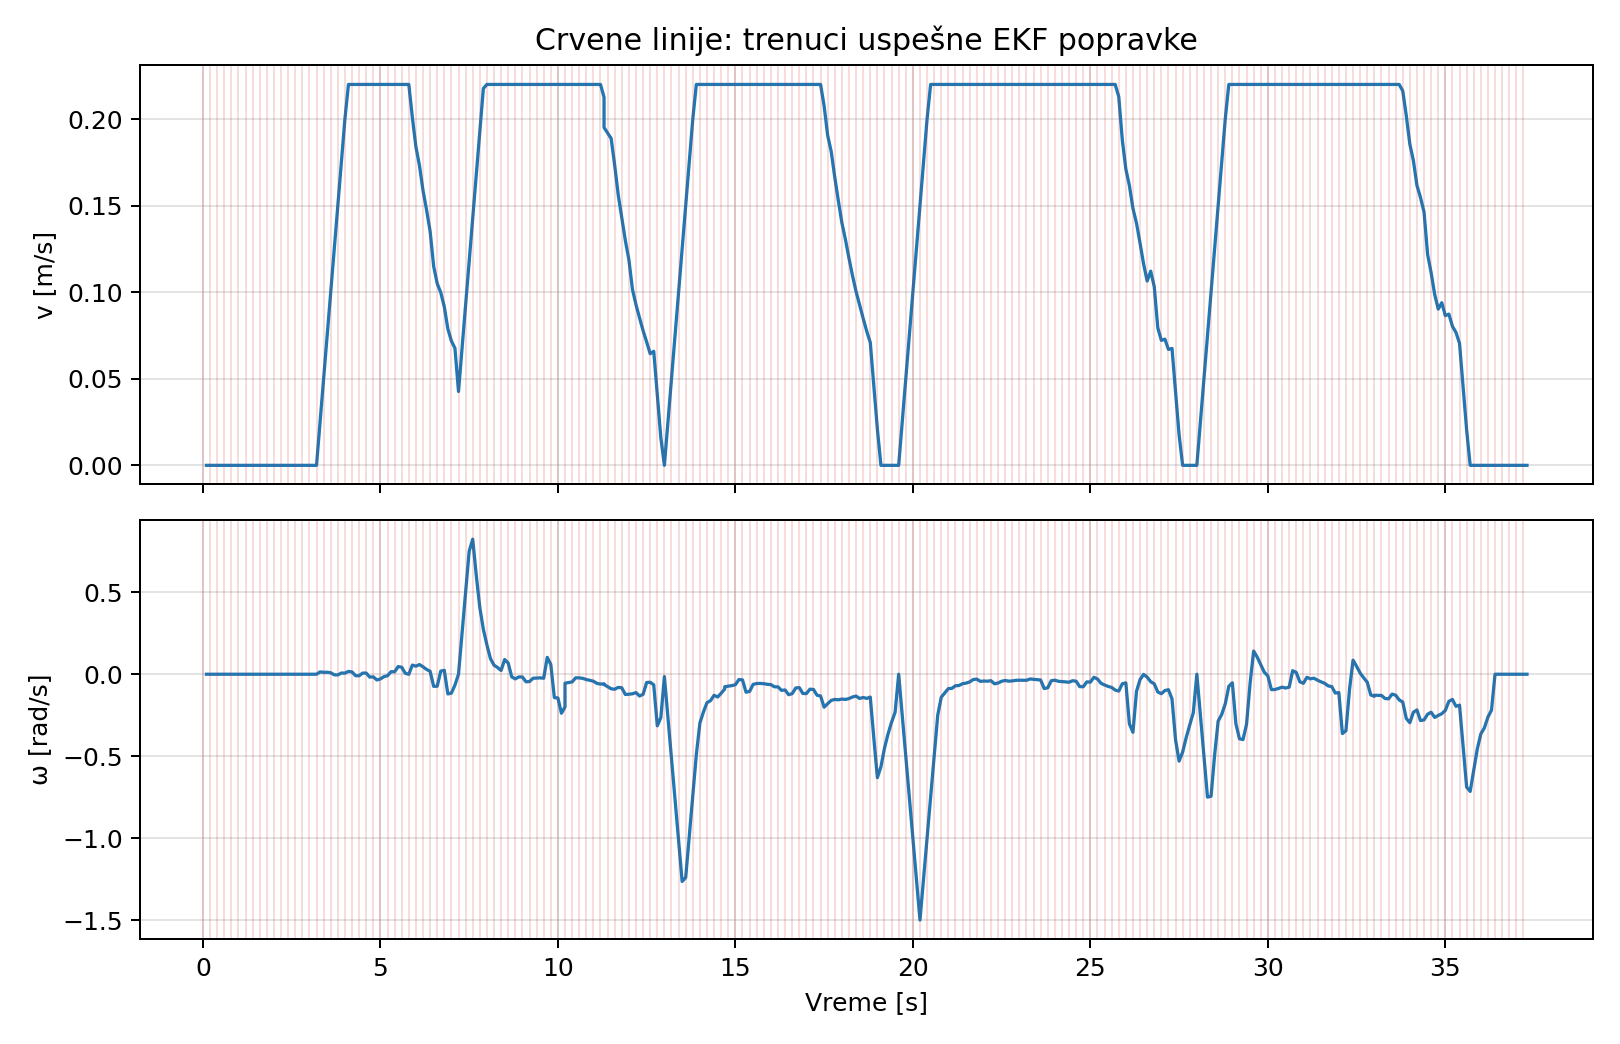
\includegraphics[width=0.92\linewidth]{results/figures/assignment7_cmd_vel_updates_b.png}
\caption{Signal /cmd\_vel u konfiguraciji (b), sa označenim trenucima EKF popravke.}
\end{figure}

U konfiguraciji (b) maksimalna apsolutna linearna brzina bila je \SI{0.220}{m/s}, a maksimalna apsolutna ugaona brzina \SI{1.500}{rad/s}. Najveći zabeleženi priraštaji između dva odbirka bili su \SI{0.025}{m/s} za linearni i \SI{0.250}{rad/s} za ugaoni kanal. Ovi brojevi su direktna posledica ograničenja brzina i rate limiting-a u regulatoru. Kada EKF popravka diskontinualno promeni estimiranu pozu, regulator vidi skok greške, ali se taj skok ne prenosi nekontrolisano na /cmd\_vel.

\subsection{Uticaj praga validacije}
\begin{figure}[h]
\centering
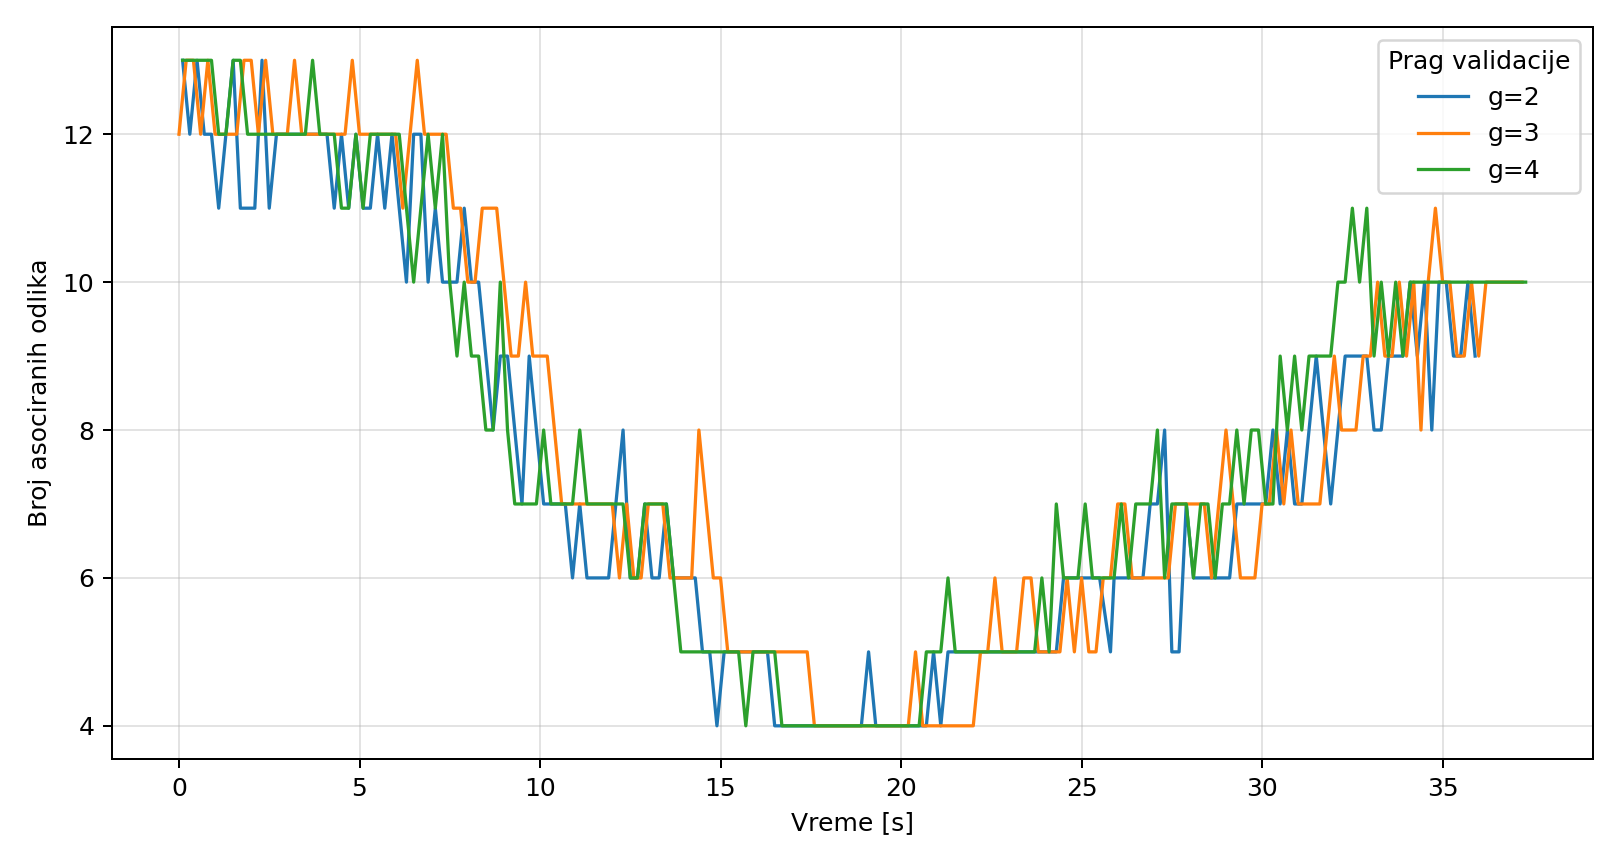
\includegraphics[width=0.92\linewidth]{results/figures/assignment7_gate_associations.png}
\caption{Broj asociranih odlika po ciklusu za različite vrednosti praga validacije $g$.}
\end{figure}

\begin{figure}[h]
\centering
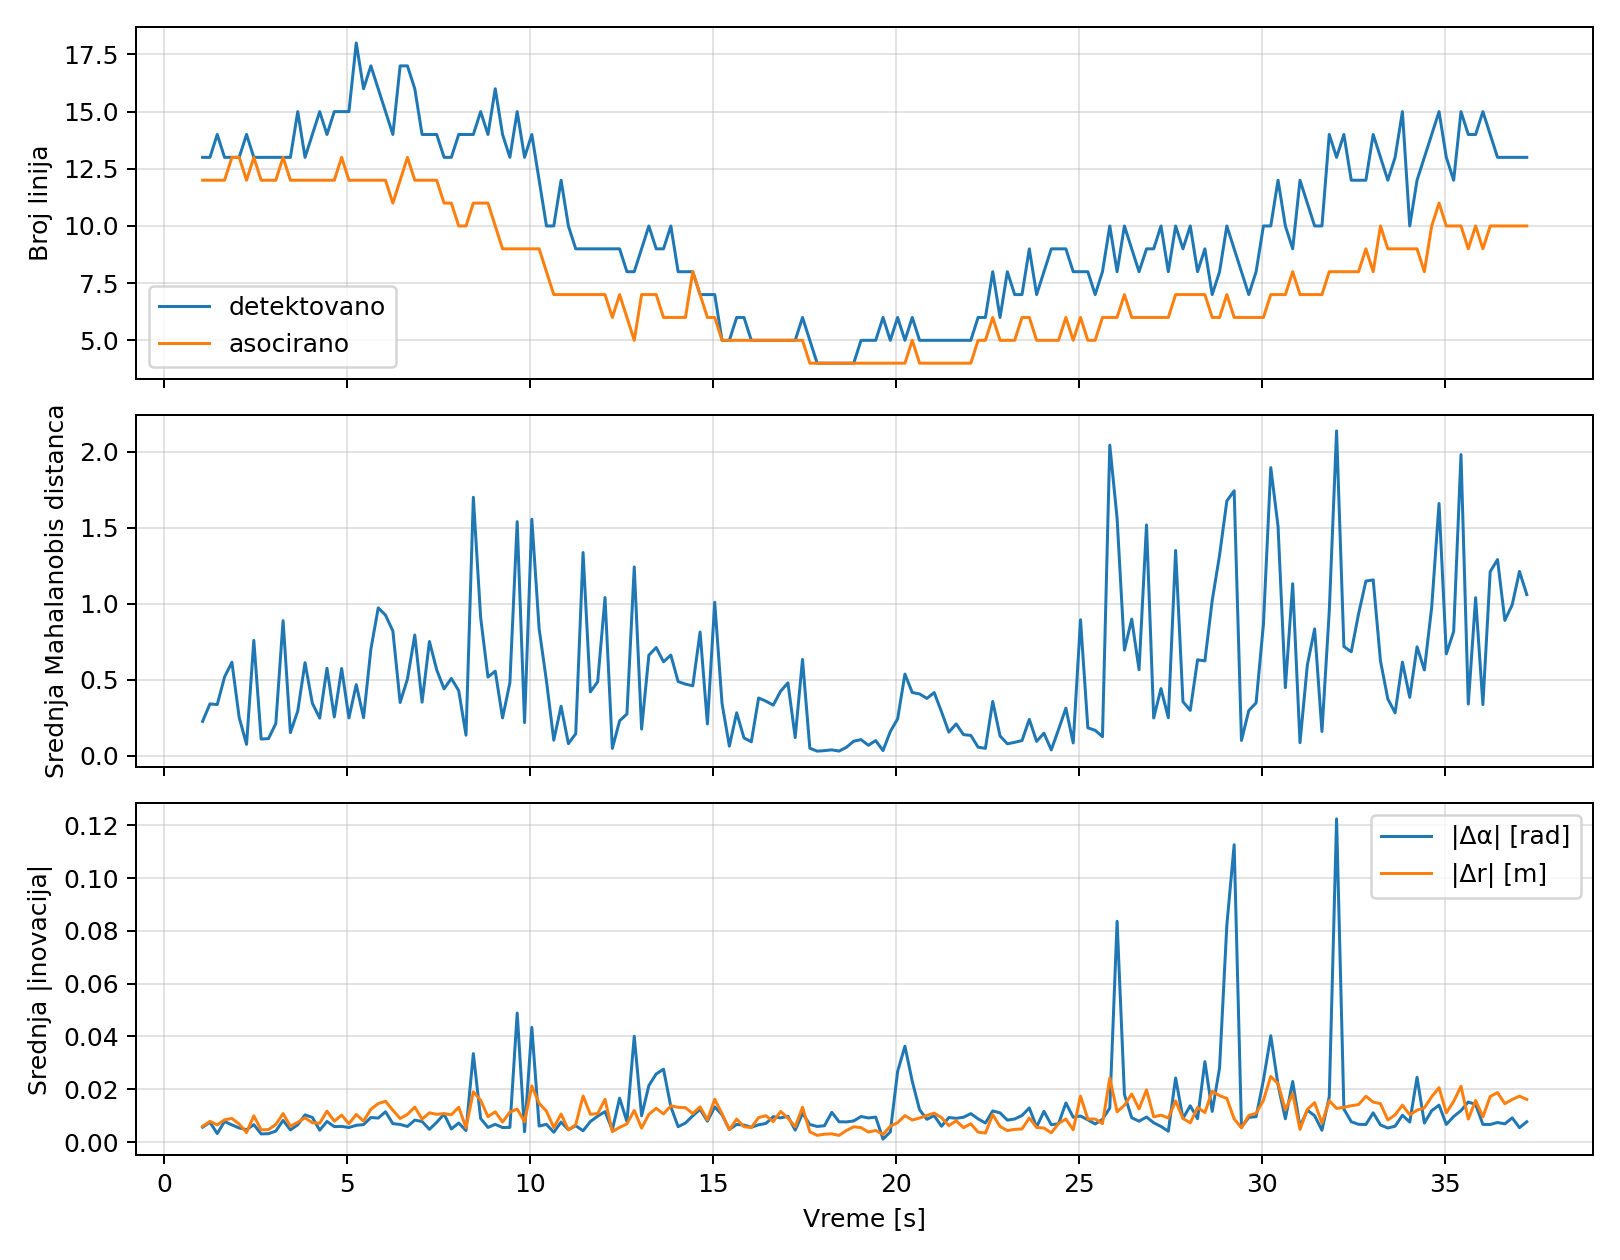
\includegraphics[width=0.92\linewidth]{results/figures/assignment7_innovation_stats.png}
\caption{Offline statistika inovacija dobijena ponovnom primenom Split-and-Merge algoritma nad /scan.}
\end{figure}

\begin{table}[h]
\centering
\begin{tabular}{rrrrr}
\hline
$g$ & Srednji broj asocijacija & Broj popravki & Srednja greška [m] & Maks. greška [m] \\
\hline
2.0 & 7.489 & 180 & 0.038 & 0.044 \\
3.0 & 7.904 & 187 & 0.040 & 0.047 \\
4.0 & 7.888 & 187 & 0.036 & 0.048 \\
\hline
\end{tabular}
\caption{Uticaj praga validacije na broj asocijacija i tačnost misije.}
\end{table}

Za $g=2$ srednji broj asociranih odlika je 7.489, za $g=3$ je 7.904, a za $g=4$ je 7.888. Manji prag zato odbacuje više opažanja i ima manji broj popravki, dok veći prag prihvata skoro isti broj merenja kao podrazumevana vrednost, ali uz potencijalno veći rizik pogrešne asocijacije. U ovim vožnjama sva tri praga daju sličnu grešku dostizanja waypoint-a, što znači da mapa i opažanja linija nisu bili u ekstremno konfliktnom režimu. Pretpostavka konstantne matrice $R$ je najslabija u delovima putanje gde su segmenti kratki, delimično zaklonjeni ili posmatrani pod oštrim uglom; tada offline statistika inovacija pokazuje povećane vrednosti $|\Delta\alpha|$, $|\Delta r|$ i Mahalanobisove distance.
